\documentclass[10pt]{article}
\usepackage{fontspec}
\setmainfont[Ligatures=TeX]{Didot}
\usepackage[utf8]{inputenc}
\usepackage[papersize={17in, 11in}]{geometry}
\usepackage[absolute]{textpos}
\TPGrid[0.5in, 0.25in]{23}{24}
\usepackage{palatino}
\parindent=0pt
\parskip=12pt
\usepackage{nopageno}
\usepackage{graphicx}
\graphicspath{ {./images/} }
\usepackage{lilyglyphs}
\usepackage{amsmath}
\begin{document}

\begin{textblock}{23}(2.667, 2)
\huge FOREWORD
\end{textblock}

\begin{textblock}{23}(10.5, 2)
\huge PREFACIO
\end{textblock}

\begin{textblock}{23}(18.333, 2)
\huge VORWORT
\end{textblock}

\begin{textblock}{7.333}(0, 3)
The string trio is a somewhat overlooked genre in contemporary music. Stemming historically from the Baroque "Trio Sonata," the string trio has a much greater relationship to the solo-against-accompaniment model of the concerto as opposed to the string quartet's more obvious relationship to the symphony orchestra. This history and the small size of the ensemble has traditionally afforded the string trio the ability to take on simultaneously a much sparser and more virtuosic character than that of the string quartet. Many composers of the common practice period of classical music used the string trio as a training ground until they were confident enough in their prowess to compose a string quartet (i.e. Mozart, Beethoven, Mendelssohn). Although the string trio has not gained a similar popularity as the string quartet, since the mid 20\textsuperscript{th} century composers have begun to establish a unique cultural role for the string trio, outside that of bourgeois, evening entertainment. The modern string trio is something beyond a beginner's string quartet. It is a genre where three independent and unique voices come together and speak in unity. \\
\phantom{text} \hfill (G.R.E.)
  \end{textblock}

\begin{textblock}{7.333}(7.8333, 3) 
El tr\'io de cuerdas es un g\'enero algo pasado por alto en la m\'usica contempor\'anea. El tr\'io de cuerdas, que viene hist\'oricamente desde el barroco "Tr\'io Sonata" tiene una relaci\'on mucho m\'as grande con el acompa�amiento en solitario para modelar el concierto como la relaci\'on obvia del cuarteto de cuerdas de orquesta sinf\'onica. Esta historia y el peque�o tama\~no del conjunto tienen tradicionalmente da el tr\'io de cuerdas, la capacidad de tomar al mismo tiempo una gran cantidad de luz y el car\'acter virtuoso como el cuarteto de cuerda. Muchos compositores de la pr\'actica de la m\'usica cl\'asica utilizaron el tr�o de cuerdas como campo de entrenamiento hasta que fueron lo suficientemente seguras como para componer un cuarteto de cuerda (es decir, Mozart, Beethoven, Mendelssohn). Aunque el tr\'io de cuerdas no haya adquirido popularidad similar a la del cuarteto de cuerda, los compositores han iniciado desde mediados del siglo 20 para establecer una funci\'on cultural \'unico para el tr\'io de cuerda fuera de la animaci\'on nocturna burgu\'es. El tr\'io de cuerdas moderno es algo m\'as que un cuarteto de cuerdas para principiantes. Es un g�nero en el que tres voces independientes y \'unicas se unen y hablan en unidad. \\
\phantom{text}  \hfill (Tr : G.R.E.)
 \end{textblock}

\begin{textblock}{7.333}(15.666, 3) 
Das Streichtrio ist ein etwas \"ubersehenes Genre in der zeitgen\"ossischen Musik. Das Streichtrio, das historisch aus der barocken "Triosonate" stammt, hat eine viel gr\"o{\ss}ere Beziehung zum Solo-gegen-Begleitung-Modell des Konzerts als das offensichtliche Verh\"altnis des Streichquartetts zum Symphonieorchester. Diese Geschichte und die geringe Gr\"o{\ss}e des Ensembles haben dem Streichtrio traditionell die F\"ahigkeit verschafft, gleichzeitig einen viel licht und virtuoseren Charakter anzunehmen als das Streichquartett. Viele Komponisten der klassischen Musikpraxis nutzten das Streichtrio als \"Ubungsplatz, bis sie selbstbewusst genug waren, ein Streichquartett zu komponieren (also Mozart, Beethoven, Mendelssohn). Obwohl das Streichtrio keine \"ahnliche Popularit\"at wie das Streichquartett erlangt hat, haben Komponisten seit Mitte des 20. Jahrhunderts begonnen, eine einzigartige kulturelle Rolle f\"ur das Streichtrio au{\ss}erhalb der bourgeois Abendunterhaltung zu etablieren. Das moderne Streichtrio ist etwas, das jenseits eines Streichquartetts f\"ur Anf\"anger liegt. Es ist ein Genre, in dem drei unabh\"angige und einzigartige Stimmen zusammenkommen und in Einheit sprechen. \\
\phantom{text} \hfill (Übs: G.R.E.)
 \end{textblock}

\begin{textblock}{23}(1.167, 12)
\huge PERFORMANCE NOTES
\end{textblock}

\begin{textblock}{23}(9, 12)
\huge NOTAS DE RENDIMIENTO
\end{textblock}

\begin{textblock}{23}(16.833, 12)
\huge LEISTUNGSHINWEISE
\end{textblock}

\begin{textblock}{7.333}(0, 13)
\pmb{Microtones}:
\end{textblock}

\begin{textblock}{23}(0, 13.5)
\includegraphics[width=0.28\textwidth]{microtones.png}
\end{textblock}

\begin{textblock}{7.333}(0, 15.5)
\pmb{String Position Staff} 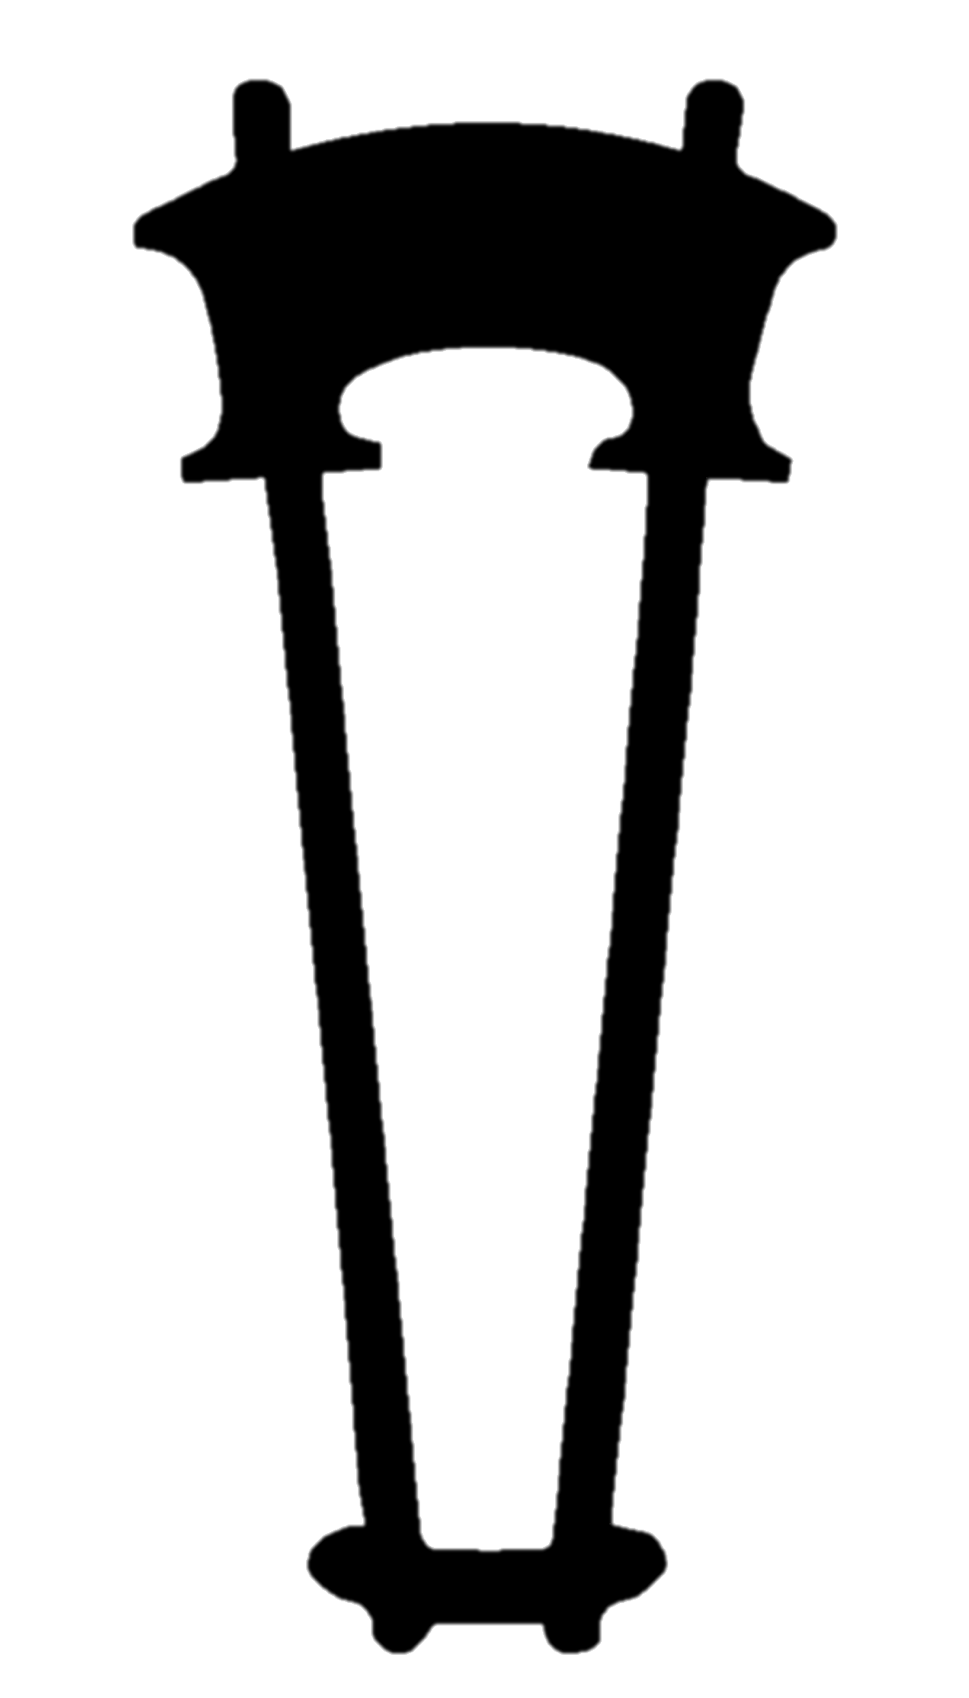
\includegraphics[width=0.02\textwidth]{string_position_tablature.eps}: The top staff for each instrument notates the vertical contact point at which the bow touches the string. These positions are written as fractions where \( \frac{0}{1} \) represents $molto \ sul tasto$ and \( \frac{1}{1} \) represents $molto \ sul \ ponticello$.

\pmb{Bow Position Staff} 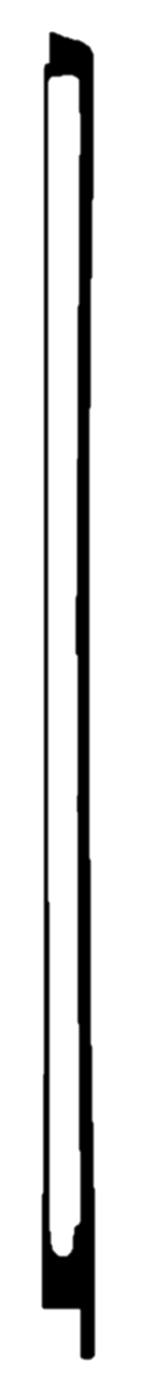
\includegraphics[height=0.025\textheight]{bow_position_tablature.eps}: The middle staff for each instrument notates the horizontal contact point at which the bow touches the string. These positions are written as fractions where \( \frac{0}{1} \) represents $au \ talon$ and \( \frac{1}{1} \) represents $punta \ d'arco$.

\pmb{MAYBE ANOTHER?} And even another technique if you have the space!.

\pmb{Four? Really?} Independantly describing four techniques may not be great...
\end{textblock}

\begin{textblock}{7.333}(7.8333, 13)
\pmb{Microtonos}:
\end{textblock}

\begin{textblock}{23}(7.8333, 13.5)
\includegraphics[width=0.28\textwidth]{microtones.png}
\end{textblock}

\begin{textblock}{7.333}(7.8333, 15.5)
\pmb{String Position Staff} 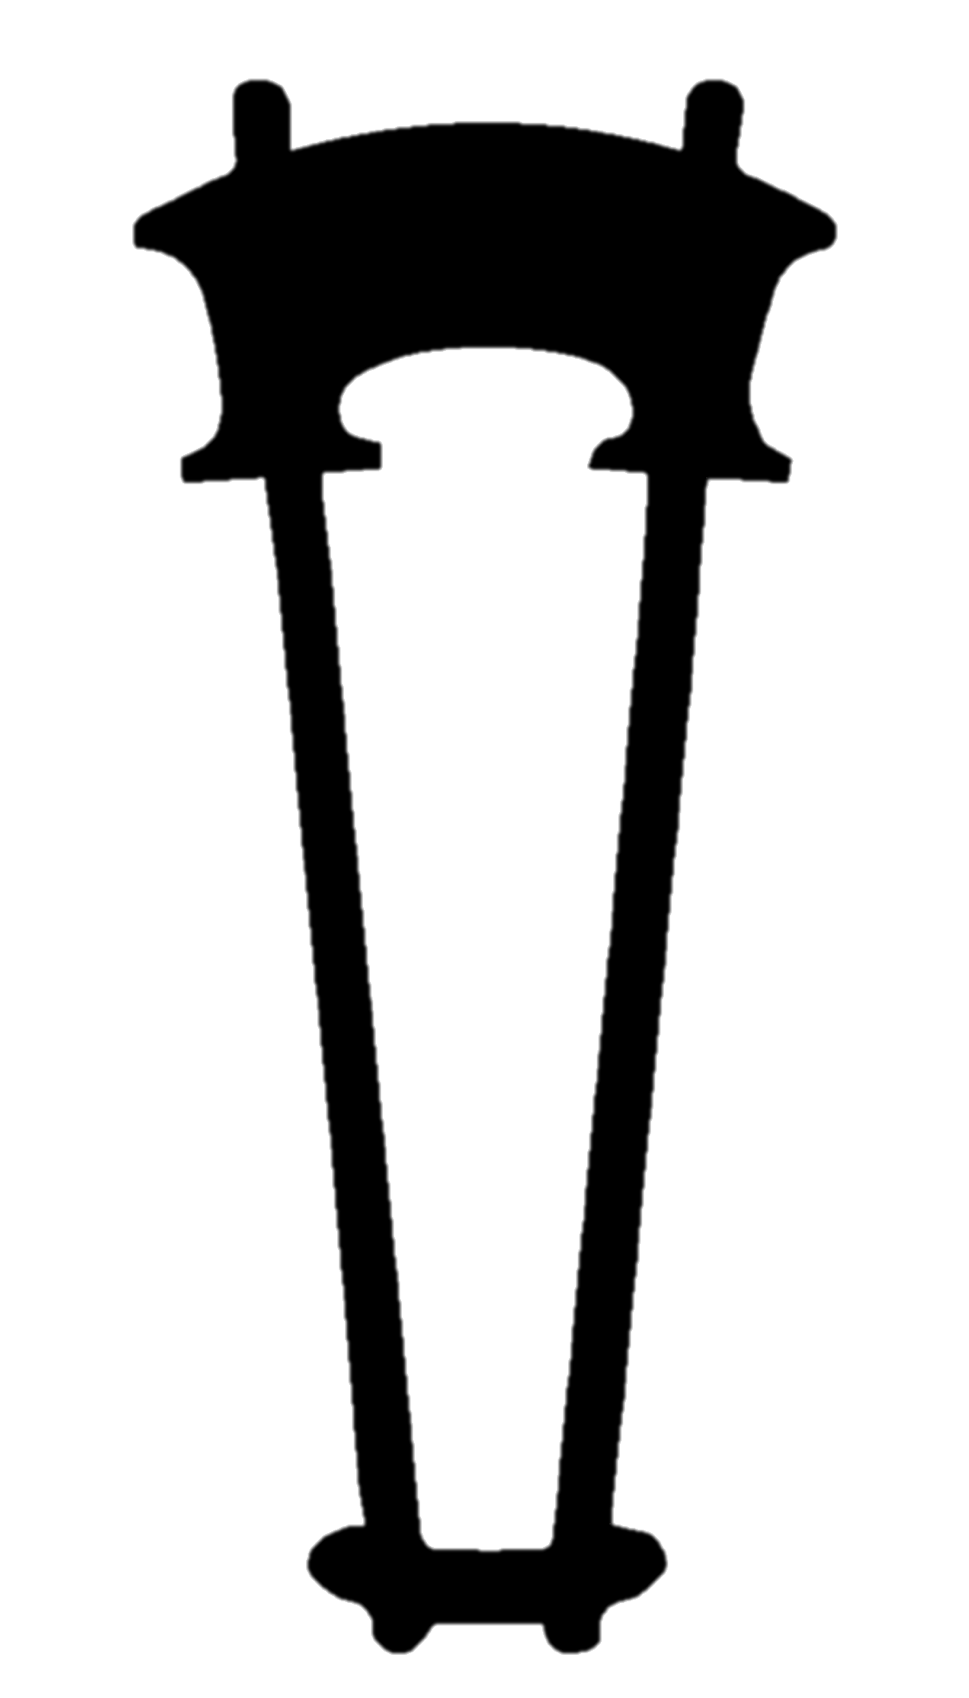
\includegraphics[width=0.02\textwidth]{string_position_tablature.eps}: The top staff for each instrument notates the vertical contact point at which the bow touches the string. These positions are written as fractions where \( \frac{0}{1} \) represents $molto \ sul tasto$ and \( \frac{1}{1} \) represents $molto \ sul \ ponticello$.

\pmb{Bow Position Staff} 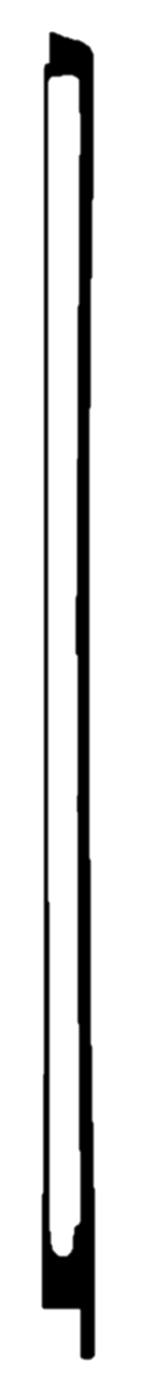
\includegraphics[height=0.025\textheight]{bow_position_tablature.eps}: The middle staff for each instrument notates the horizontal contact point at which the bow touches the string. These positions are written as fractions where \( \frac{0}{1} \) represents $au \ talon$ and \( \frac{1}{1} \) represents $punta \ d'arco$.

\pmb{MAYBE ANOTHER?} And even another technique if you have the space!.

\pmb{Four? Really?} Independently describing four techniques may not be great...
\end{textblock}

\begin{textblock}{7.333}(15.666, 13)
\pmb{Mikrotonalen Intervallen}:
\end{textblock}

\begin{textblock}{23}(15.666, 13.5)
\includegraphics[width=0.28\textwidth]{microtones.png}
\end{textblock}

\begin{textblock}{7.333}(15.666, 15.5)
\pmb{String Position Staff} 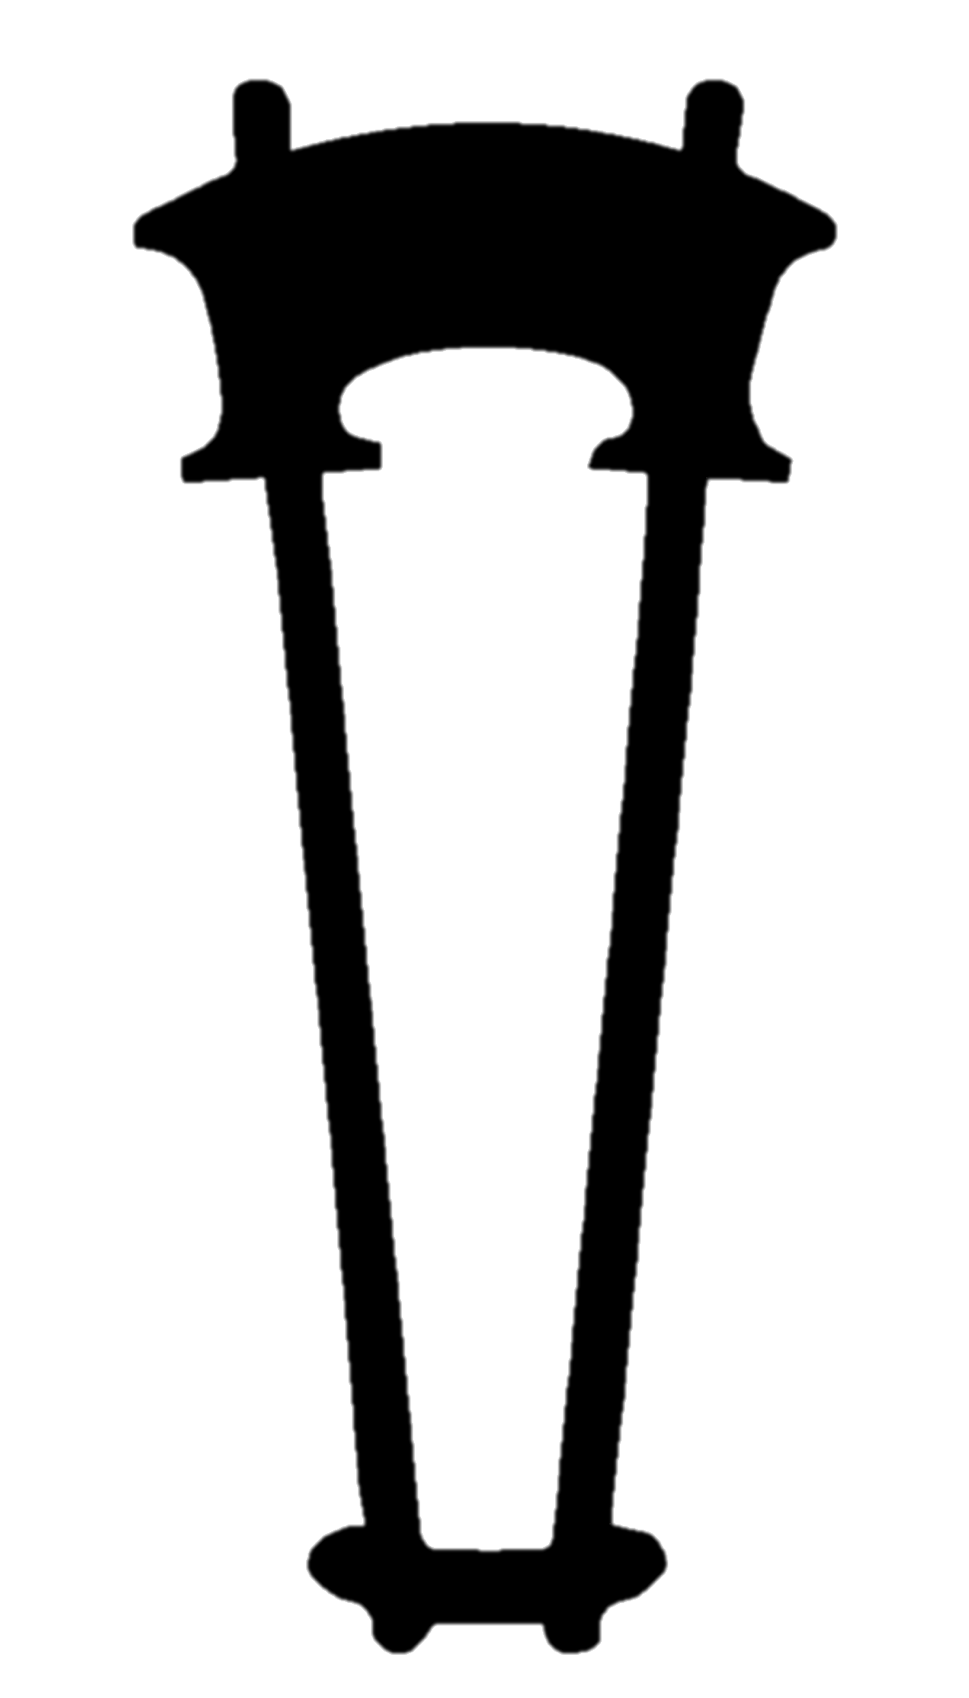
\includegraphics[width=0.02\textwidth]{string_position_tablature.eps}: The top staff for each instrument notates the vertical contact point at which the bow touches the string. These positions are written as fractions where \( \frac{0}{1} \) represents $molto \ sul \ tasto$ and \( \frac{1}{1} \) represents $molto \ sul \ ponticello$.

\pmb{Bow Position Staff} 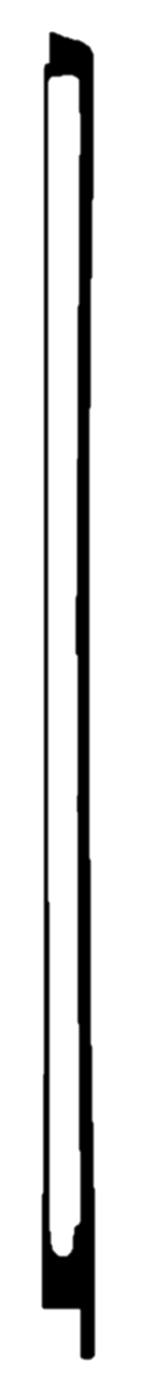
\includegraphics[height=0.025\textheight]{bow_position_tablature.eps}: The middle staff for each instrument notates the horizontal contact point at which the bow touches the string. These positions are written as fractions where \( \frac{0}{1} \) represents $au \ talon$ and \( \frac{1}{1} \) represents $punta \ d'arco$.

\pmb{MAYBE ANOTHER?} And even another technique if you have the space!.

\pmb{Four? Really?} Independantly describing four techniques may not be great...
\end{textblock}

\begin{textblock}{7.333}(0, 23)
$Adumbration$ is dedicated in admiration and friendship to Trevor Ba\v{c}a, Josiah Wolf Oberholtzer, and Jeffrey Trevi\~{n}o from whom I have learned so much.
\end{textblock}

\begin{textblock}{7.333}(7.8333, 23)
$Adumbration$ is dedicated in admiration and friendship to Trevor Ba\v{c}a, Josiah Wolf Oberholtzer, and Jeffrey Trevi\~{n}o from whom I have learned so much.
\end{textblock}

\begin{textblock}{7.333}(15.666, 23)
$Adumbration$ is dedicated in admiration and friendship to Trevor Ba\v{c}a, Josiah Wolf Oberholtzer, and Jeffrey Trevi\~{n}o from whom I have learned so much.
\end{textblock}

\end{document}